Es gibt  drei Parameter  zu evaluieren: Das Massentr\"agheitsmoment  $I_0$ der
Apparatur ohne Reiter,  die Periodendauer $T_0$ f\"ur  kleine Auslenkungen und
die Federkonstante $k$. Die numerischen Resultate  f\"ur $I_0$ sind in Tabelle
\ref{tab:resultsI0}  zu  finden;  Abbildung  \ref{fig:resultsI0}  zeigt  einen
graphischen Vergleich der verschiedenen Methoden.

\begin{table}[h!]
    \centering
    \caption{Ergebnisse f\"ur $I_0$ via verschiedene Methoden}
    \label{tab:resultsI0}
    \begin{tabular}{p{70mm}r}
        \toprule
        Methode                                                                 & Resultat \\
        \midrule
        Versuch 3.1.1                                                           & \SI{12.03 \pm 0.02}{\gram\meter\squared} \\
        Versuch 3.1.2, Reiter als Punktmasse approximiert                       & \SI{11.4 \pm 0.4}{\gram\meter\squared} \\
        Versuch 3.1.2, Reiter als Zylinder modelliert                           & \SI{11.3 \pm 0.4}{\gram\meter\squared} \\
        Versuch 3.1.2, Reiter als Zylinder modelliert, eingeengter Fit-Bereich  & \SI{12.31 \pm 0.09}{\gram\meter\squared} \\
        Referenz Versuchsanleitung                                              & \SI{11.6}{\gram\meter\squared} \\
        \bottomrule
    \end{tabular}
\end{table}

\begin{figure}[ht!]
\centering
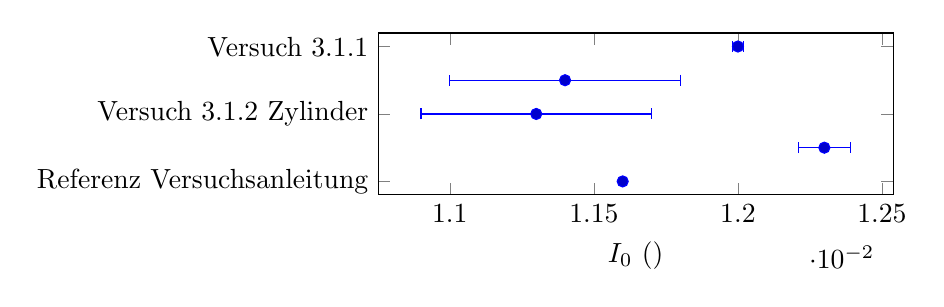
\begin{tikzpicture}
    \begin{axis}[
        width=.67\textwidth,
        height=.3\textwidth,
        %title = {Eisengehalt},
        xlabel = {$I_0$ ($\si{\kilo\gram\meter\squared}$)},
        %symbolic y coords = {ungewichtet,gewichtet, QtiPlot gewichtet},
        symbolic y coords = {Referenz Versuchsanleitung,Versuch 3.1.2 Zylinder 2,Versuch 3.1.2 Zylinder,Versuch 3.1.2 Punktmasse,Versuch 3.1.1},
    ]
    \addplot+[
        only marks,error bars/.cd,
        x dir=both,x explicit,
        error bar style={line width=0.5pt},
        ]
    coordinates {
        (1.20e-2,Versuch 3.1.1) +- (1.9e-5,0)
        (1.14e-2,Versuch 3.1.2 Punktmasse) +- (4e-4,0)
        (1.13e-2,Versuch 3.1.2 Zylinder) +- (4e-4,0)
        (1.23e-2,Versuch 3.1.2 Zylinder 2) +- (9e-5,0)
        (1.16e-2,Referenz Versuchsanleitung) +- (0,0)
    };
    \end{axis}
\end{tikzpicture}
\caption{graphische Darstellung der Ergebnisse zum f\"ur $I_0$}
\label{fig:resultsI0}
\end{figure}

F\"ur  die  Periode   $T_0$  beim  Schwerependel  ergaben   sich  zwei  Werte,
einer  f\"ur  den vollen  Messbereicht,  und  einer  aus  dem Fit  \"uber  den
eingeschr\"ankten  Wertebereich. Die  entsprechenden  Werte  sind  in  Tabelle
\ref{tab:resultsT0} respektive Abbildung \ref{fig:resultsT0} zu finden.

T\begin{table}[h!]
    \centering
    \caption{Ergebnisse f\"ur $T_0$ des Schwerependels}
    \label{tab:resultsT0}
    \begin{tabular}{p{70mm}r}
        \toprule
        Versuch                         & Resultat \\
        \midrule
        voller Messbereich              & \SI{1.403 \pm 0.006}{\second} \\
        eingeschr\"ankter Wertebereich  & \SI{1.419 \pm 0.002}{\second} \\
        \bottomrule
    \end{tabular}
\end{table}

\pgfplotsset{try min ticks=2}
\begin{figure}[ht!]
\centering
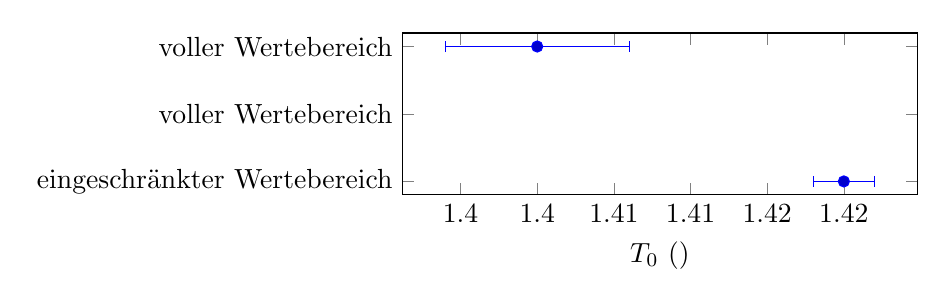
\begin{tikzpicture}
    \begin{axis}[
        width=.67\textwidth,
        height=.3\textwidth,
        %title = {Eisengehalt},
        xlabel = {$T_0$ ($\si{\second}$)},
        %symbolic y coords = {ungewichtet,gewichtet, QtiPlot gewichtet},
        symbolic y coords = {eingeschr\"ankter Wertebereich,voller Wertebereich},
    ]
    \addplot+[
        only marks,error bars/.cd,
        x dir=both,x explicit,
        error bar style={line width=0.5pt},
        ]
    coordinates {
        (1.40,voller Wertebereich) +- (0.006,0)
        (1.42,eingeschr\"ankter Wertebereich) +- (0.002,0)
    };
    \end{axis}
\end{tikzpicture}
\caption{graphische Darstellung der Ergebnisse zum f\"ur $T_0$ beim Schwerependel}
\label{fig:resultsT0}
\end{figure}

Zu   guter  Letzt   werden   in  Tabelle   \ref{tab:resultsk}  und   Abbildung
\ref{fig:resultsk} noch die Werte f\"ur die Federkonstante $k$ dargestellt und
verglichen.

\begin{table}[h!]
    \centering
    \caption{Ergebnisse f\"ur $k$ via verschiedene Methoden}
    \label{tab:resultsk}
    \begin{tabular}{p{70mm}r}
        \toprule
        Methode       & Resultat \\
        \midrule
        Versuch 3.3.1 & \SI{32.0   \pm  0.2}{\newton\per\meter} \\
        Versuch 3.3.2 & \SI{30.917 \pm  0.007}{\newton\per\meter} \\
        Versuch 3.3.3 & \SI{29.95 \pm  0.07}{\newton\per\meter} \\
        Referenzwert  & \SI{32.0}{\newton\per\meter} \\
        \bottomrule
    \end{tabular}
\end{table}

\pgfplotsset{try min ticks=4}
\begin{figure}[ht!]
\centering
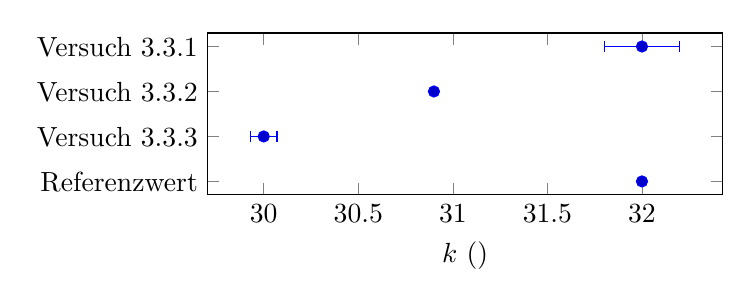
\begin{tikzpicture}
    \begin{axis}[
        width=.67\textwidth,
        height=.3\textwidth,
        %title = {Eisengehalt},
        xlabel = {$k$ ($\si{\newton\per\meter}$)},
        symbolic y coords = {Referenzwert,Versuch 3.3.3,Versuch 3.3.2,Versuch 3.3.1},
    ]
    \addplot+[
        only marks,error bars/.cd,
        x dir=both,x explicit,
        error bar style={line width=0.5pt},
        ]
    coordinates {
        (32.0,Referenzwert) +- (0,0)
        (32.0,Versuch 3.3.1) +- (0.2,0)
        (30.9,Versuch 3.3.2) +- (0.007,0)
        (30.0,Versuch 3.3.3) +- (0.07,0)
    };
    \end{axis}
\end{tikzpicture}
\caption{graphische Darstellung der Ergebnisse zum f\"ur $k$}
\label{fig:resultsk}
\end{figure}


Alles   in  Allem   beurteile  ich   die  Ergebnisse   zufriedenstellent,  mit
Ausnahme  des  Fits  in  Abschnitt  \ref{subsubsec:kombiP:auslvar}  auf  Seite
\pageref{subsubsec:kombiP:auslvar},   welcher  aus   mir  bisher   unbekannten
Gr\"unden nicht wirklich stimmt (zumindest soweit ich dies beurteilen kann).
